\documentclass[9pt]{beamer}


\usepackage{multirow}
\usepackage{graphics} 
\usepackage[french]{babel} 
\usepackage{ucs}
\usepackage[utf8x]{inputenc} 
\usepackage{pgfpages}
\usepackage[absolute,overlay]{textpos}
%\setbeameroption{show notes on second screen} 
%\pgfpagesuselayout{2 on 1}[a4paper,landscape]
%\pgfpagesuselayout{two screens with optional second}



\title[7Robot \hspace{0.1cm}Présentation du club]{Présentation du club} 
%\author[7Robot]{7Robot}           
\institute{ ENSEEIHT}

% ------------- modif du thème
\usetheme{Warsaw}
\setbeamertemplate{navigation symbols}{}
\setbeamertemplate{headline}
{%
  \leavevmode
  \begin{beamercolorbox}[wd=.5\paperwidth,ht=2.5ex,dp=1.125ex,leftskip=.3cm plus1fill,rightskip=.3cm]{section in head/foot}%
    \insertsection
  \end{beamercolorbox}%
  \begin{beamercolorbox}[wd=.5\paperwidth,ht=2.5ex,dp=1.125ex,leftskip=.3cm,rightskip=.3cm plus1fil]{subsection in head/foot}%
    \insertsubsection
  \end{beamercolorbox}%
}
\addtobeamertemplate{headline}
{}
{%
  \vskip-0.2pt
  \pgfuseshading{beamer@topshade}
  \vskip-2pt
}

\setbeamertemplate{footline}{
\leavevmode%
\hbox{\hspace*{-0.06cm}
\begin{beamercolorbox}[wd=.2\paperwidth,ht=2.25ex,dp=1ex,center]{author in head/foot}%
	\usebeamerfont{author in head/foot}\insertshortauthor%~~(\insertshortinstitute)
\end{beamercolorbox}%
\begin{beamercolorbox}[wd=.6\paperwidth,ht=2.25ex,dp=1ex,center]{section in head/foot}%
	\usebeamerfont{section in head/foot}\insertshorttitle
\end{beamercolorbox}%
\begin{beamercolorbox}[wd=.2\paperwidth,ht=2.25ex,dp=1ex,right]{section in head/foot}%
	%\usebeamerfont{section in head/foot}\insertshortdate{}\hspace*{2em}
	\insertframenumber{} / \inserttotalframenumber\hspace*{2ex}
\end{beamercolorbox}}%
\vskip0pt%
}

\setbeamertemplate{section in toc}
{\inserttocsectionnumber. ~ \inserttocsection \\}

\setbeamertemplate{subsection in toc}
{\hspace{0.5cm} \inserttocsubsectionnumber. ~ \inserttocsubsection \\}

\setbeamertemplate{subsubsection in toc}
{\hspace{1cm} \inserttocsubsubsectionnumber. ~ \inserttocsubsubsection \\}

\newcommand\bottom[1]{%
  \begin{textblock*}{\textwidth}(1cm,\textheight-1cm)%
    #1
  \end{textblock*}
}



\begin{document}



%##############################################################
%                            TITRE
%##############################################################


%%------------  TITRE  ------------
\begin{frame}
	\frametitle{}
	
	\begin{center}
		
\includegraphics[width=0.5\textwidth]{logo}
	\end{center}
	
	\vspace{-1.2cm}
	
	\titlepage
	
\end{frame}

{
  \begin{frame}
    \frametitle{Plan}
    \tableofcontents[currentsection,currentsubsection]
  \end{frame}
}


%% ############################# Le club ############################
\section[Le club]{Le club}

%%------------ 7Robot  ------------
\begin{frame}
	\frametitle{7Robot}
	\begin{itemize}
		\item Le club de robotique de l'ENSEEIHT
		\item Un local en E117 avec du matériel
		\item Des membres dynamiques et passionnés
		\item Différents projets, dont la Coupe de France		
	\end{itemize}
	
	\vspace{0.3cm}
	
	\begin{center}
		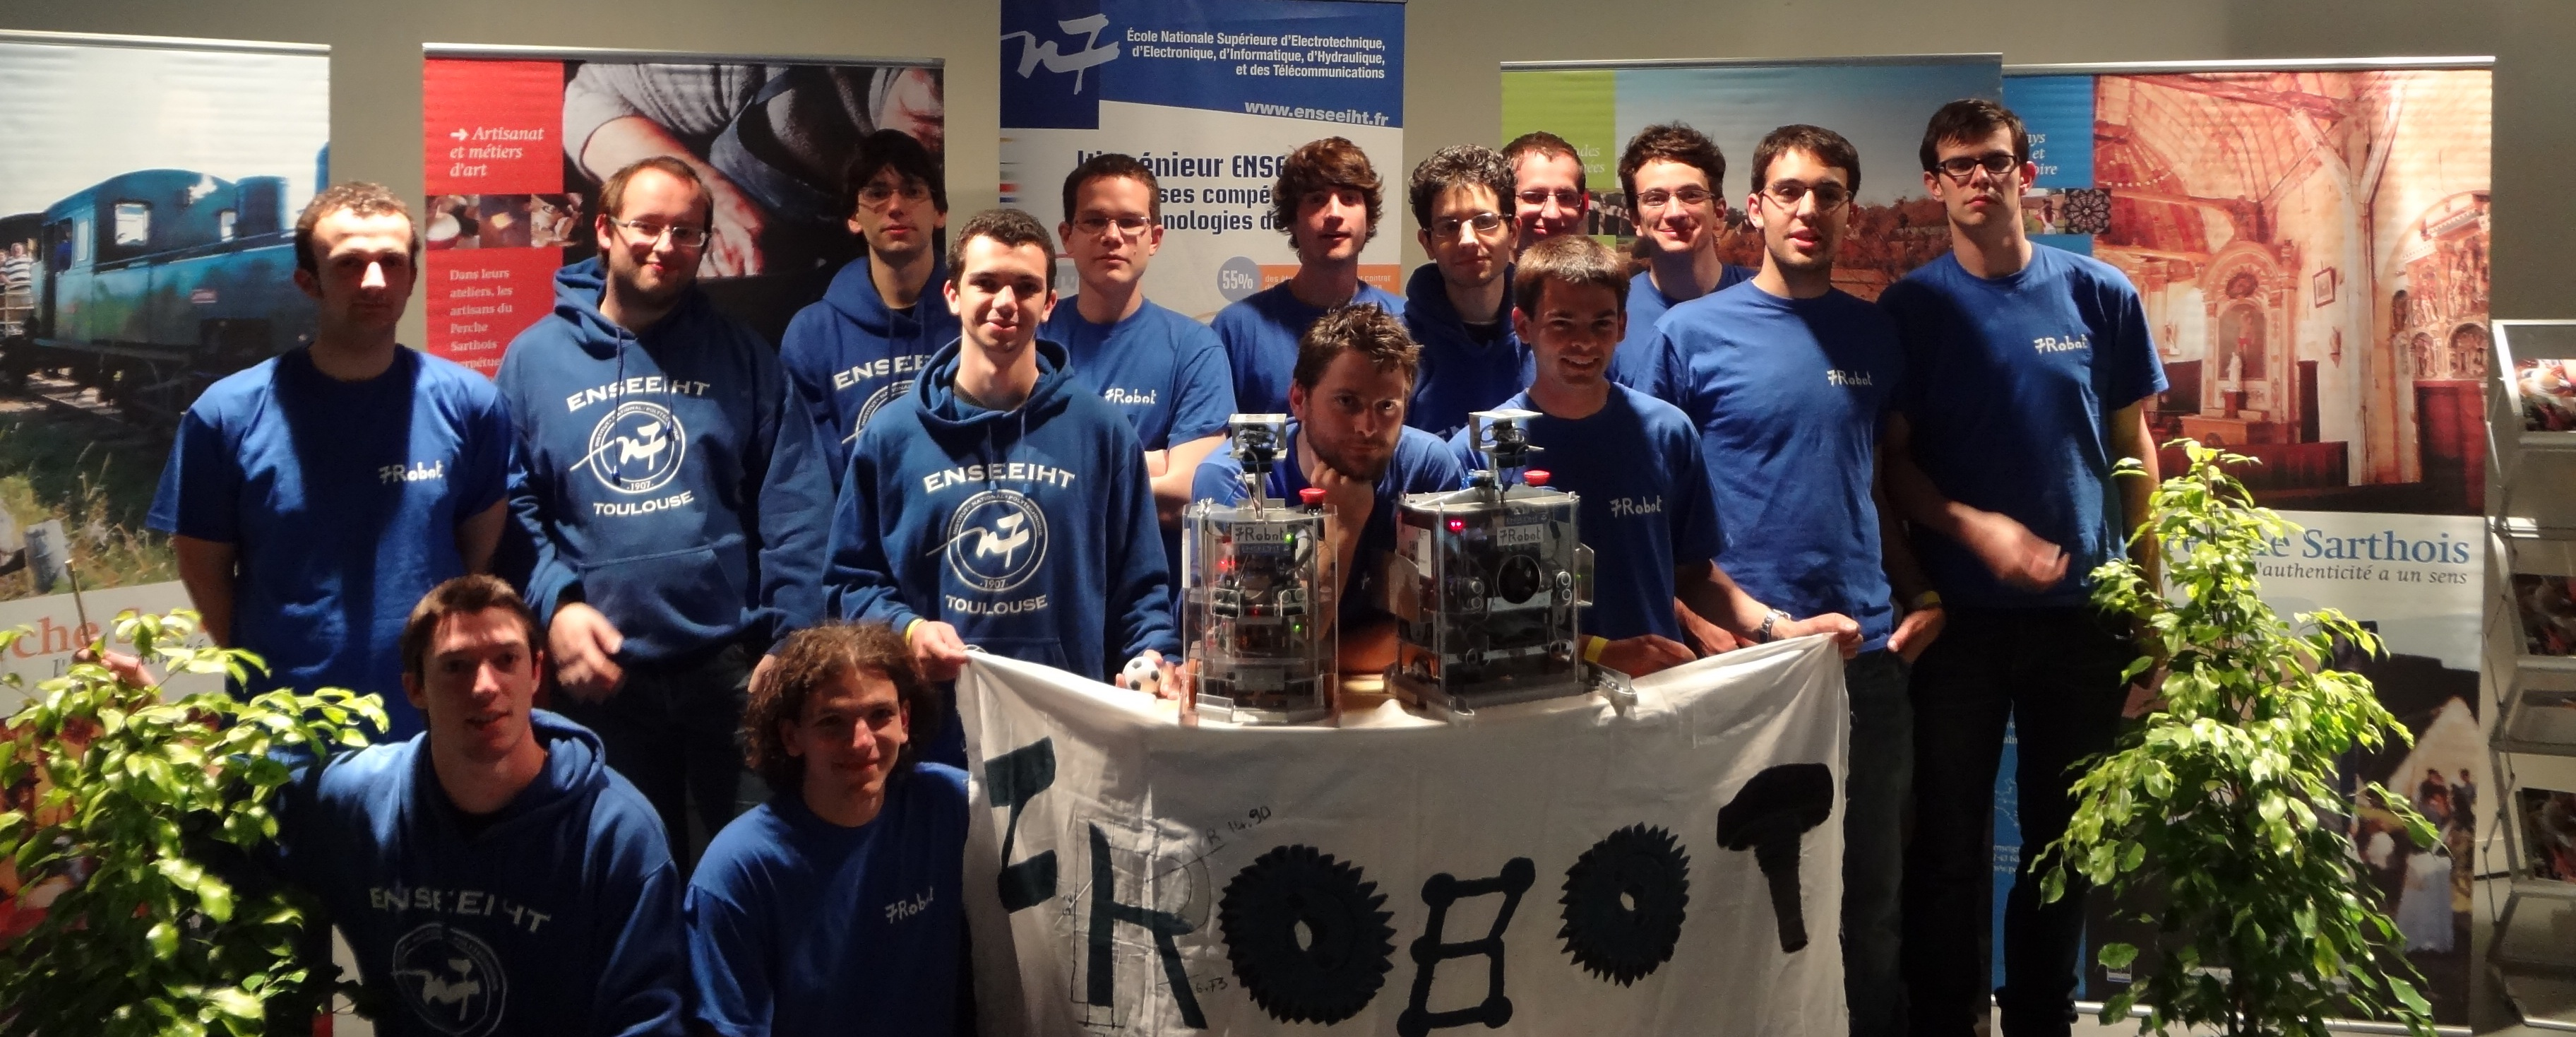
\includegraphics[width=0.95\textwidth]{groupe}
	\end{center}

\end{frame}

%%------------ Organisation du club  ------------
\begin{frame}
	\frametitle{Organisation du club}
	
	
	\begin{tabular}{ r l }
	   Président : & Ken Hasselmann \\
	   Vice-président : & Élie Bouttier  \\
	   Trésorier : & Guillaume Dib  \\
	   Secrétaire : & Thomas Nicot  \\
	\end{tabular}

	\begin{itemize}
		\item Le travail a lieu dans le local pendant notre temps libre
		\item Les membres travaillent en groupe
		\item Les réunions s'organisent grâce à la liste de diffusion
	\end{itemize}

\end{frame}


%% ############################# Activités ############################

\section{Nos Activités}

%%------------ A l'N7 ------------
\begin{frame}
	\frametitle{À l'ENSEEIHT}
	

	\begin{tabular}{ l l }
		\begin{minipage}[c]{.4\linewidth}
			Électronique diverse pour l'école.
		\end{minipage} &  
		\begin{minipage}[c]{.6\linewidth}
			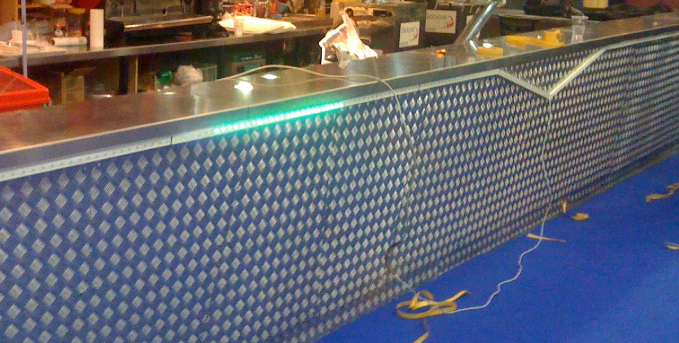
\includegraphics[width=.9\textwidth]{bar}
		\end{minipage}\\
	\end{tabular}
	
	\begin{tabular}{ l l }
		\begin{minipage}[c]{.4\linewidth}
			Diverses formations : Arduino, PICs, \ldots
		\end{minipage} &  
		\begin{minipage}[c]{.6\linewidth}
			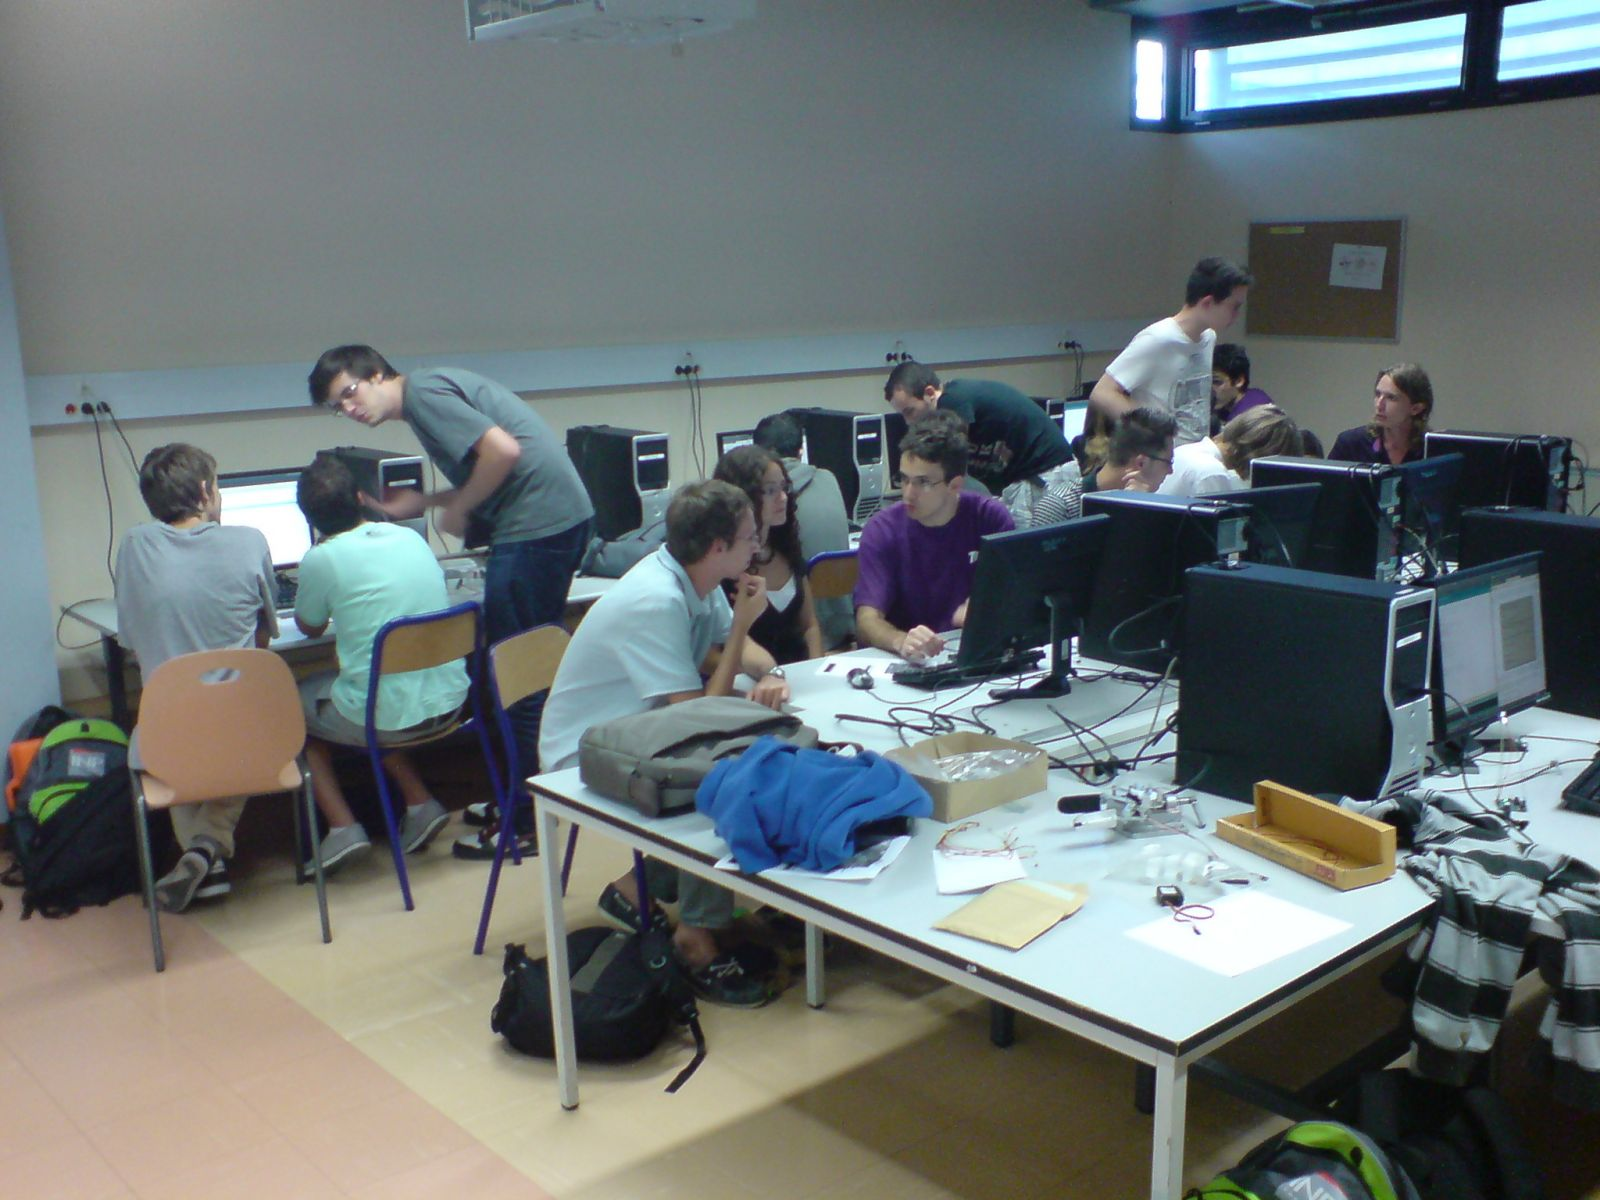
\includegraphics[width=0.9\textwidth]{formation}
		\end{minipage}\\
	\end{tabular}
	

		
		
		

	
\end{frame}

%%------------ AOC Michelet  ------------
\begin{frame}
	\frametitle{AOC Michelet}
	
	\begin{center}
		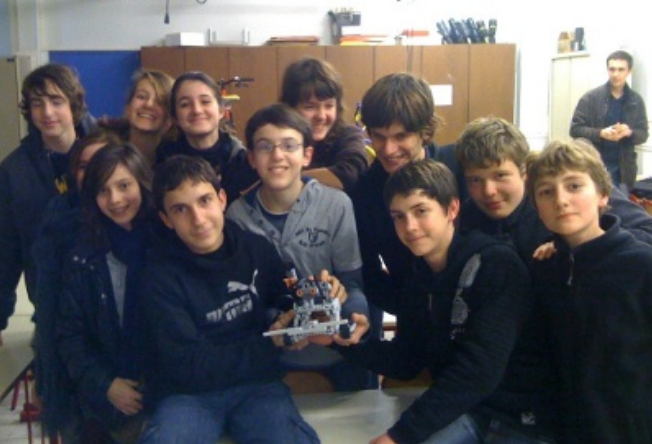
\includegraphics[width=0.5\textwidth]{michelet}
		
		Initiations à la robotique au collège Michelet

	\end{center}
	
\end{frame}


%%------------ RobAFIS  ------------
\begin{frame}
	\frametitle{RobAFIS}
	
	\begin{center}
		
\includegraphics[width=0.5\textwidth]{logo_robafis}
		
		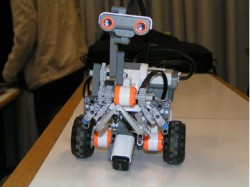
\includegraphics[width=0.5\textwidth]{robafis}
	\end{center}

\end{frame}

%%------------ Freescale  ------------
\begin{frame}
	\frametitle{Freescale}
	
	\begin{center}
		
\includegraphics[width=0.5\textwidth]{freescale}
	\end{center}
	
	\vspace{1cm}
	
	\begin{tabular}{ l l }
		\begin{minipage}[c]{.5\linewidth}
			\begin{itemize}    
				\item Processeur, DSP et chassis fournis   
				\item Course de suiveurs de ligne   
				\item Départ annulé suite aux grèves des controlleurs aériens     
			\end{itemize}
		\end{minipage} &  
		\begin{minipage}[c]{.5\linewidth}
			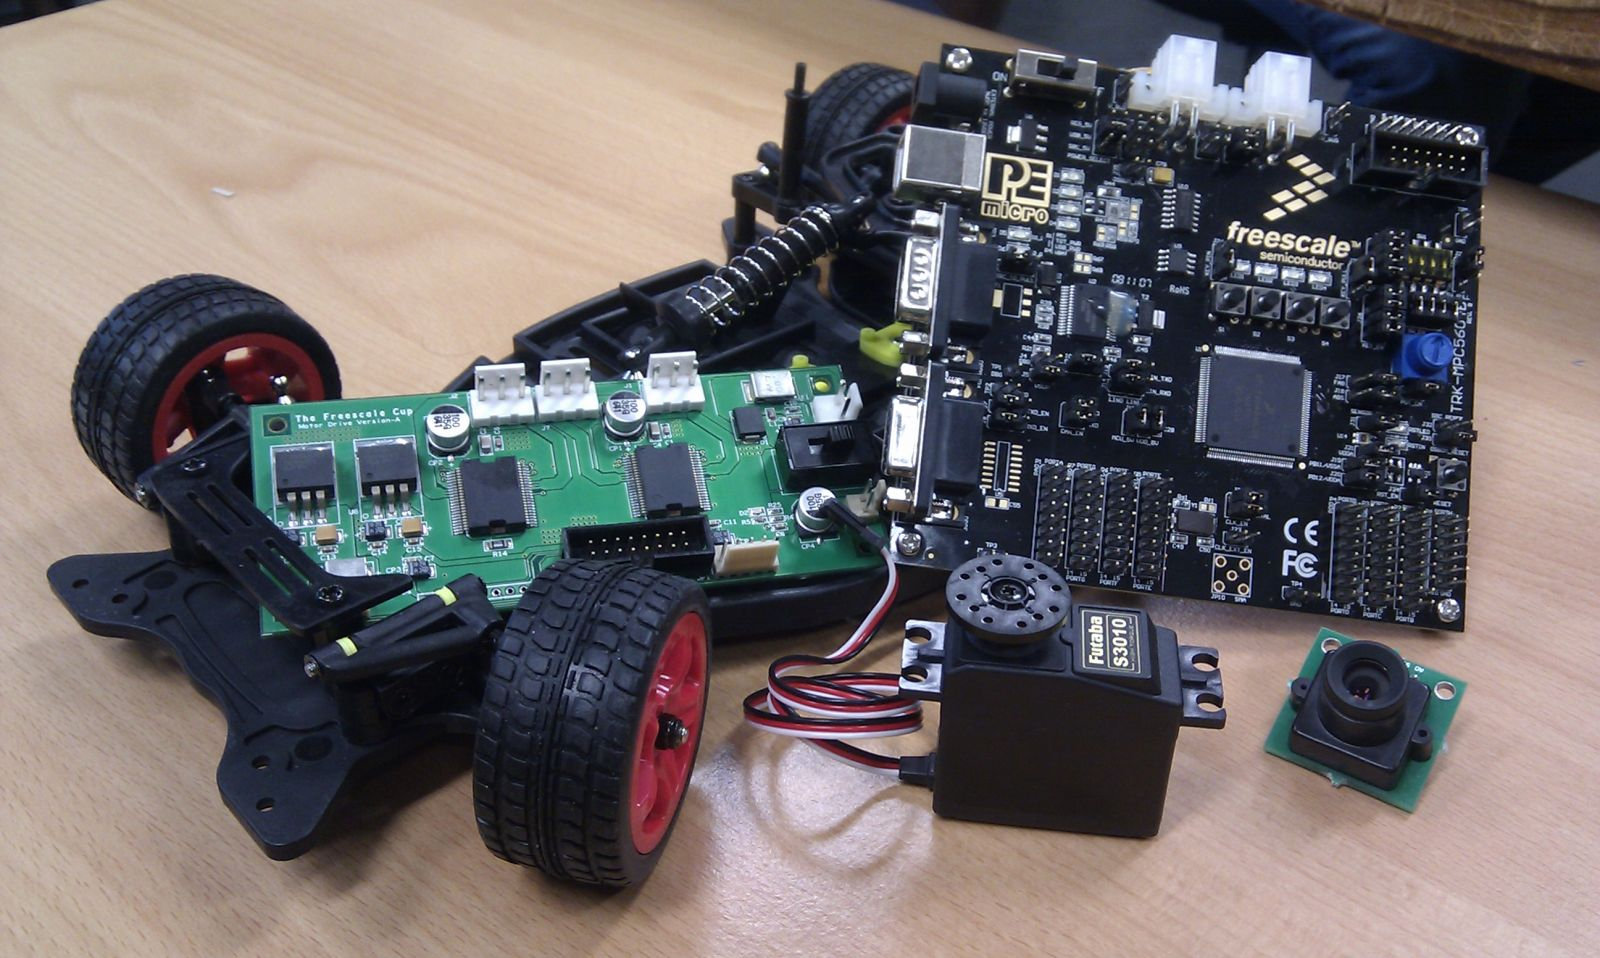
\includegraphics[width=\textwidth]{freescale-kit} 
		\end{minipage}\\

	\end{tabular}
	
	

%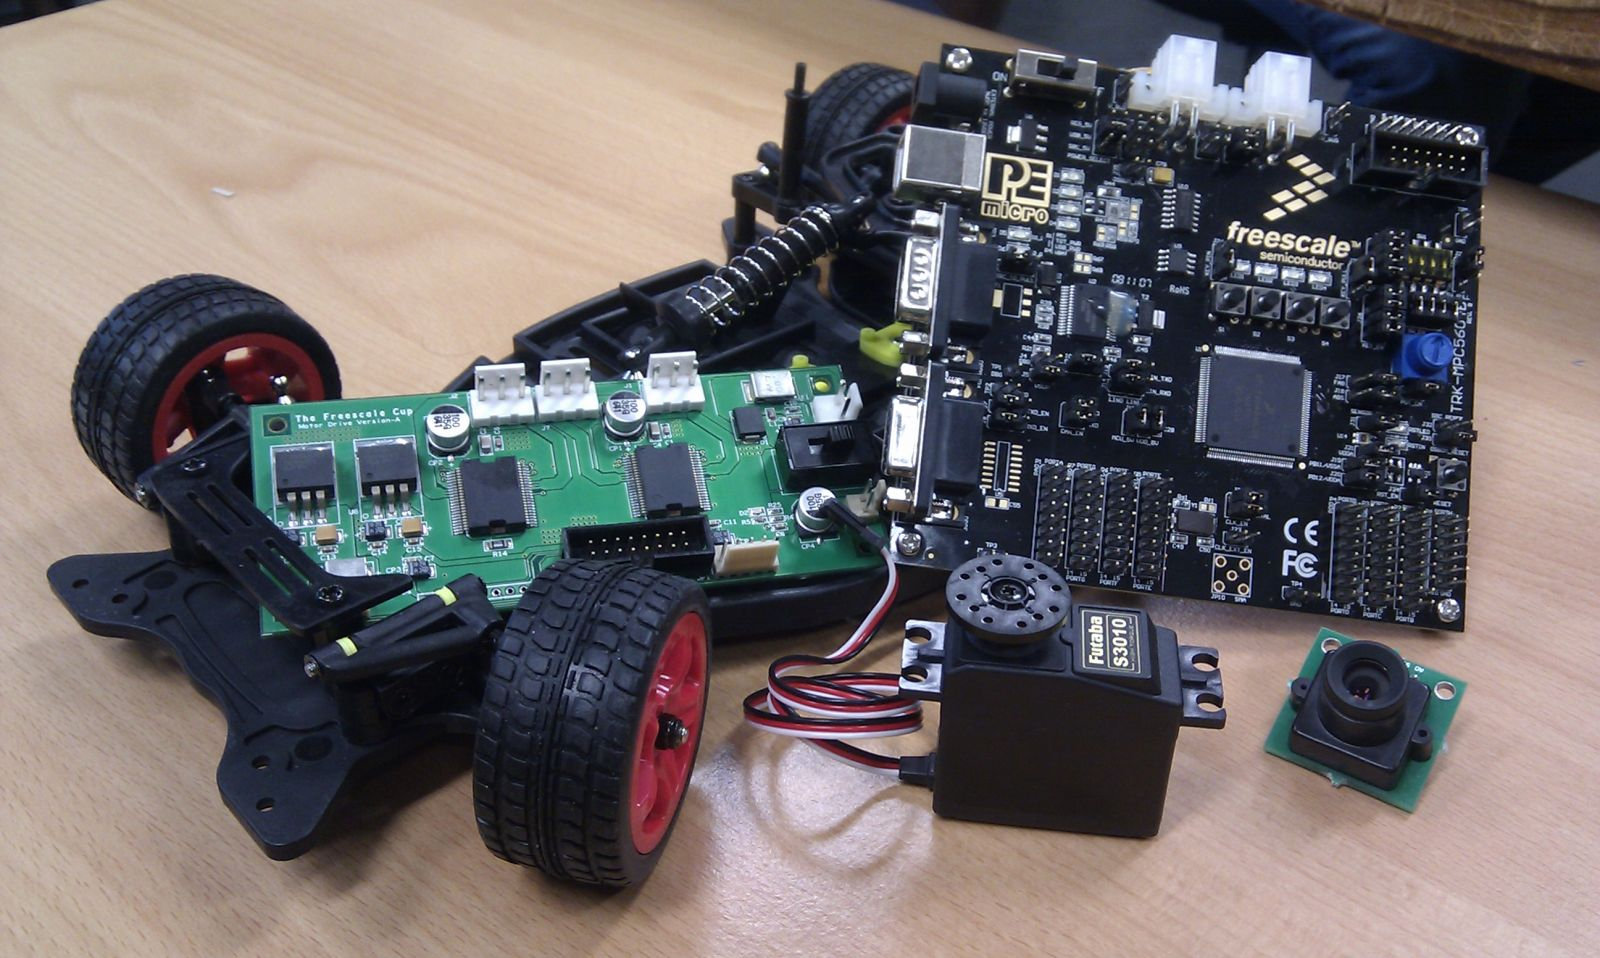
\includegraphics[width=0.5\textwidth]{freescale-kit}
\end{frame}


%%------------ Coupe de France  ------------
\begin{frame}
	\frametitle{Coupe de France}
	
	\begin{center}
		
\includegraphics[width=0.25\textwidth]{treasure-island}
		\hspace{0.5cm}
		
\includegraphics[width=0.5\textwidth]{cdf}
	\end{center}
	
	\begin{itemize}
		\item 180 équipes, en majorité des élèves ingénieurs
		\item Une année de préparation
		\item 4 jours à la Ferté-Bernard (près du Mans)
	\end{itemize}

\end{frame}


\begin{frame}
	\frametitle{Coupe de France}
	\begin{itemize}
		\item 60èmes en 2010
		\item 44èmes en 2011
		\item 24èmes en 2012
	\end{itemize}
	
	\vspace{1cm}
	
	\begin{center}
		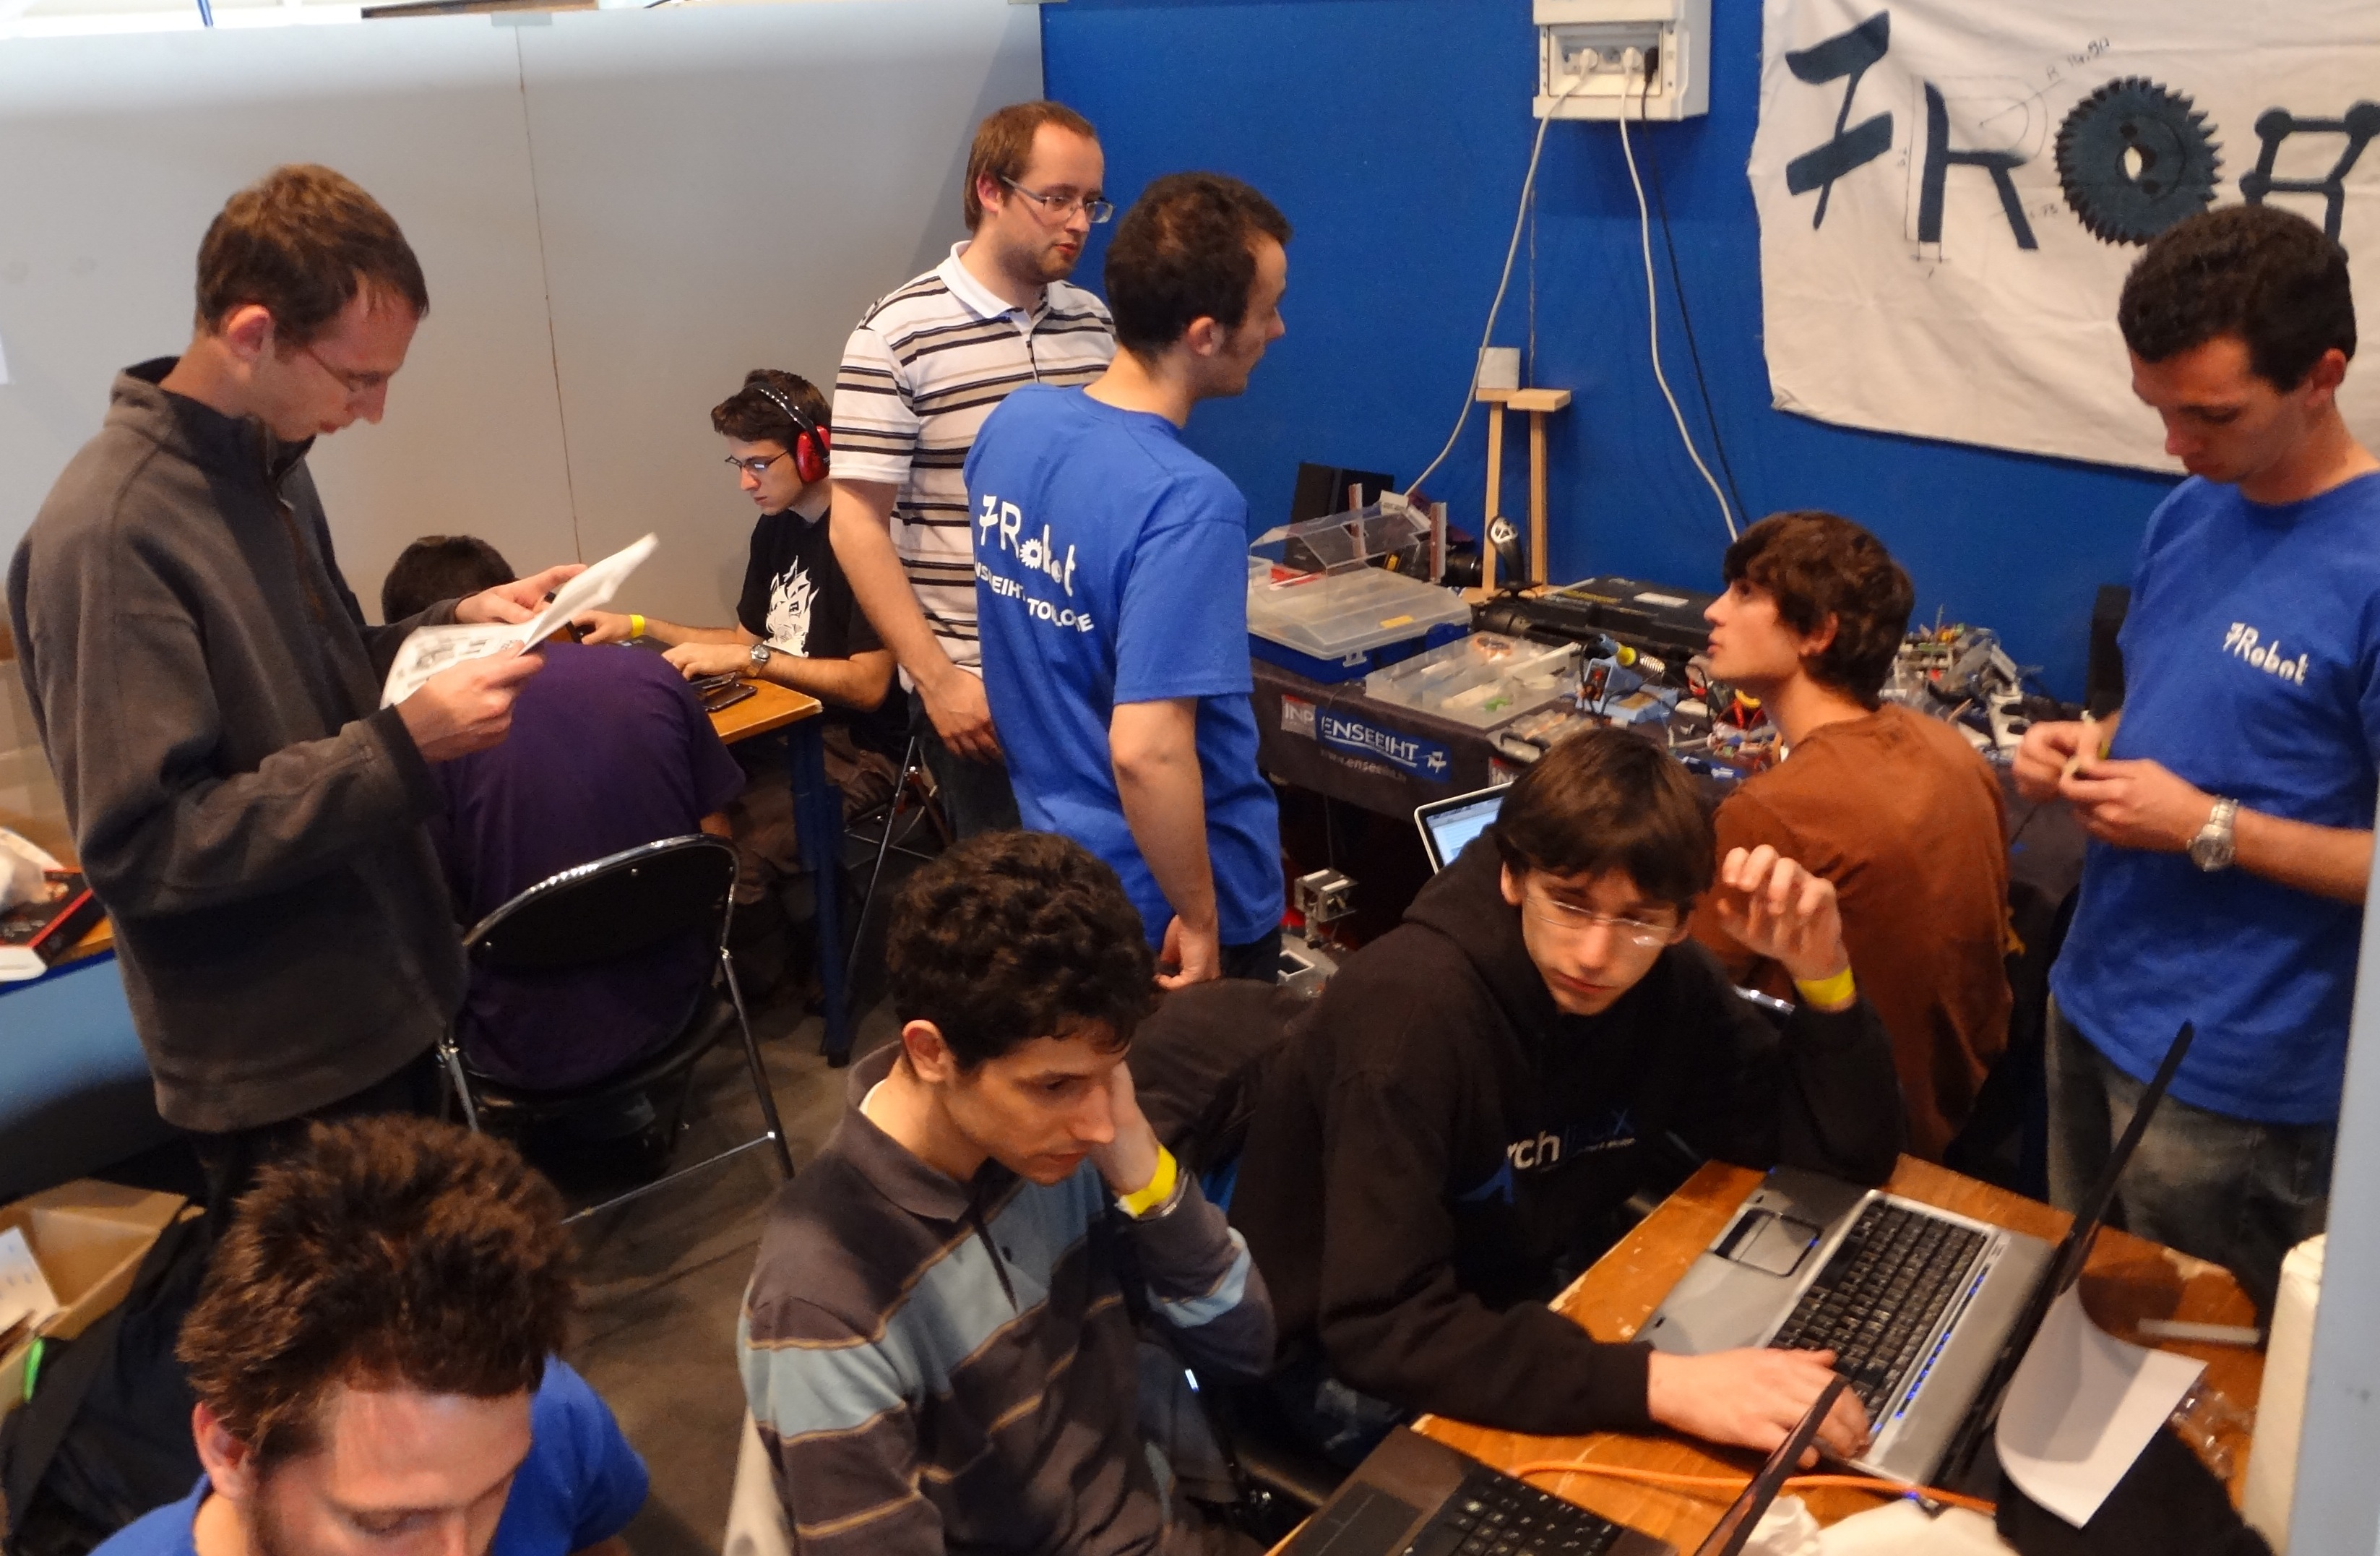
\includegraphics[height=0.4\textheight]{cdf_travail}
		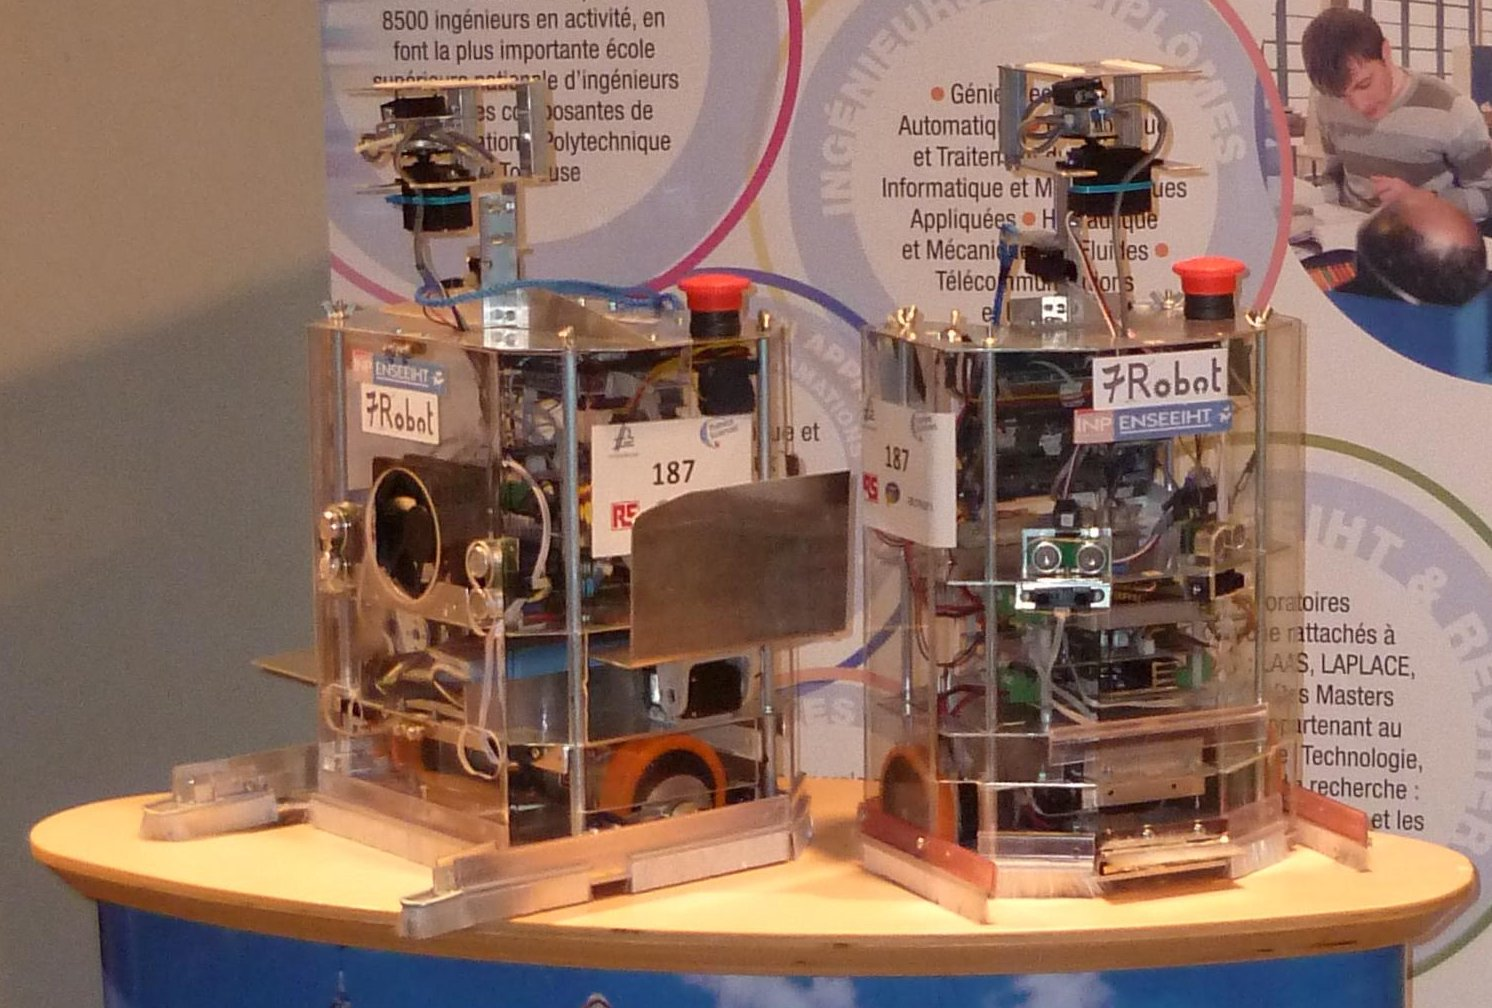
\includegraphics[height=0.4\textheight]{cdf_robots}
	\end{center}

\end{frame}

%%------------ Le prochain robot  ------------
\begin{frame}
	\frametitle{Le prochain robot}
	
	\begin{tabular}{ l l }
		\begin{minipage}[c]{.5\linewidth}
			\begin{itemize}
				\item Usinage à commande numérique
				\item CMS
				\item Rasberry Pi
				\item Moteurs 24V
				\item Capteurs infra-rouge
				\item dsPICs et PICs 33F
			\end{itemize}
		\end{minipage} &  
		\begin{minipage}[c]{.5\linewidth}
			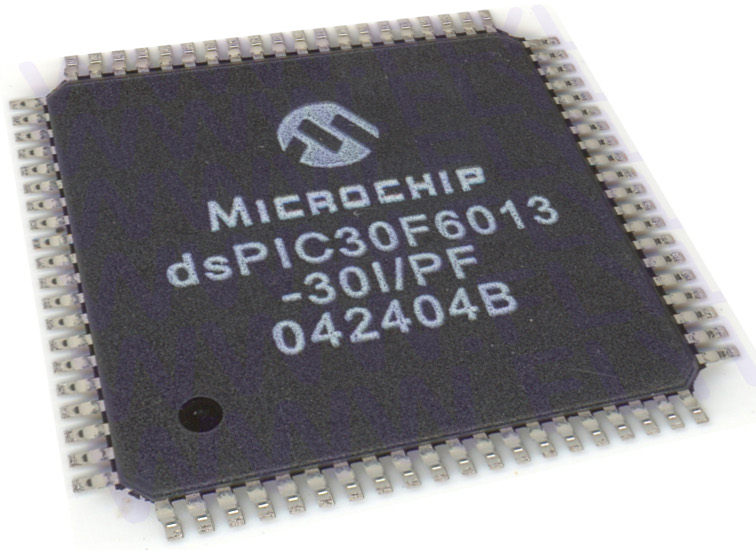
\includegraphics[width=0.4\textwidth]{dspic} \\
			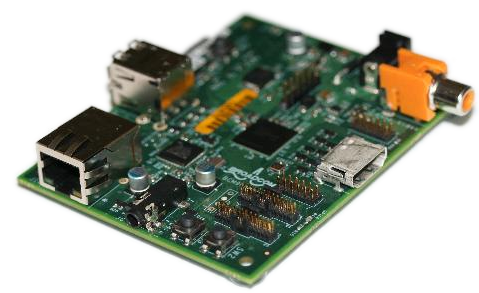
\includegraphics[width=0.7\textwidth]{rasberry_pi} 
		\end{minipage}\\

	\end{tabular}

	
	
\end{frame}


%% ############################# Conclusion ############################

\section{Conclusion}

%%------------ CONCLUSION  ------------
\begin{frame}
	\frametitle{Conclusion}
	
	\begin{itemize}
		\item Un club dynamique et plein d'idées
		\item Un complément au cursus classique	
		\item Une mise en valeur de l'école dans chacun de nos projets
	\end{itemize}
\end{frame}

%%------------ MERCI  ------------
\begin{frame}
	\frametitle{Merci}
	
	\begin{center}
		
\includegraphics[width=0.5\textwidth]{logo}
	\end{center}
	
	\begin{tabular}{ r l }
		Site web : &	\texttt{http://bde.enseeiht.fr/clubs/robot/} \\
		Contact :  &	\texttt{7robot@bde.enseeiht.fr} \\
	\end{tabular}
	


	\begin{center}
		\bottom{
\includegraphics[height=0.08\textheight]{logo_n7}
				\hspace{0.2cm}
				
\includegraphics[height=0.08\textheight]{logo_ed}
			    \hspace{0.2cm}
				
\includegraphics[height=0.08\textheight]{arcelor-mittal}
		}
	\end{center}

\end{frame}


\end{document}
